\section{WebRouteMap Design}
\label{sec:neighbors}

\subsection{Framework Overview}

\begin{figure*}[t]
\centering
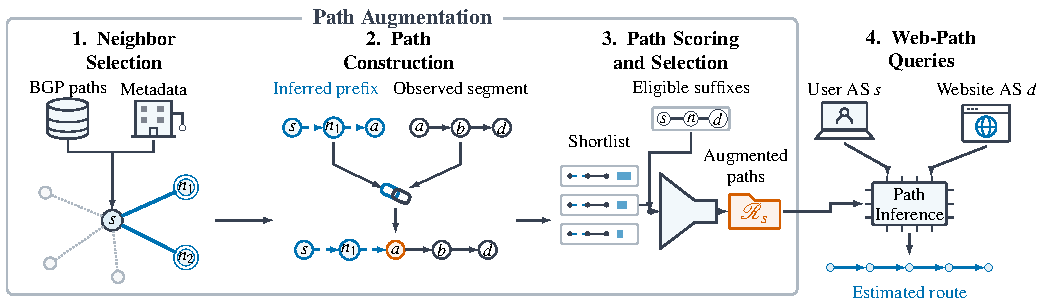
\includegraphics[width=\textwidth]{figures/fig2_overview.pdf}
\caption{\sys groups the first three steps as path augmentation, producing
a library for model training and Web-path queries. Dashed prefixes join
solid observed segments; observed suffixes enter the shared scoring and
selection stage.}
\Description{The first three scenes are enclosed in a frame labeled Path
Augmentation: neighbor selection, path construction by joining a prefix to
an observed segment, and path scoring and selection into a shared library.
The fourth scene, outside the frame, answers user-to-website path queries.}
\label{fig:overview}
\end{figure*}

\sys estimates the routes behind Web access using a source-specific path
library $\mathcal R_s$ constructed from other networks' observations and
public interconnection information. For each source and snapshot, learned
neighbor ranking and recursive exploration identify usable branches.
Stitching reuses observed segments; complete-path scoring and selection
admit candidates into the library.

Figure~\ref{fig:overview} separates path augmentation (Steps~1--3) from website queries. Shared
AS, transition, and path representations support the construction decisions.
The selected library supplies training paths and local evidence for
candidate generation, and is reused across website endpoints.

\subsection{Representing Public Routing Evidence}
\label{sec:evidence_representation}

We encode AS relationships, graph structure, network attributes,
PeeringDB co-location, and observed paths as tabular features at three
levels (Table~\ref{tab:method_features})~\cite{CAIDA,caidaASrank,PeeringDB}.
Provenance and missing or conflicting evidence remain explicit.
Co-location supplies candidate information without establishing adjacency.

\begin{table}[t]
\centering
\caption{Public evidence at AS, transition, and path levels, complemented
by destination context and uncertainty indicators.}
\label{tab:method_features}
\small
\begin{tabularx}{\columnwidth}{@{}lX@{}}
\toprule
Level & Representation and use\\
\midrule
AS and AS pair & Network size and transit role; graph connectivity and
overlap; shared PeeringDB locations. Used to rank possible neighbors.\\
Transition & Preceding, current, and next AS; directed commercial roles,
local support, and prefix-phase compatibility. Used for exploration and
prefix assessment.\\
Complete path & Ordered edge and segment support, prefix reliability,
actual third AS, and continuation evidence. Used to score constructed
routes.\\
Destination context & Donor agreement toward the same destination, with
incoming-role conditioning and equal donor-source weighting; evaluated
at the first hop and stitching boundary.\\
Uncertainty & Missing metadata, unknown or conflicting roles, absent
donor coverage, and the end of a construction boundary.\\
\bottomrule
\end{tabularx}
\end{table}


\paragraph{Destination-conditioned routing support.}
An observed route at a neighbor need not be available to the source:
learning, selecting, and exporting a BGP route are distinct
operations~\cite{rfc4271}. For a candidate $(s,n,a,\ldots,d)$, we therefore
measure whether other source networks observe $n$ followed by $a$ toward
the same destination $d$. Let $c_v(n,a,d)$ count distinct observed paths
beginning $(v,n,a)$ and ending at $d$, and let
$c_v(n,d)=\sum_b c_v(n,b,d)$. With
$V_{n,d}=\{v:c_v(n,d)>0\}$, we compute
\begin{equation}
\begin{split}
f(n,a,d)&=\frac{|\{v\in V_{n,d}:c_v(n,a,d)>0\}|}{|V_{n,d}|},\\
m(n,a,d)&=\frac{1}{|V_{n,d}|}\sum_{v\in V_{n,d}}
                    \frac{c_v(n,a,d)}{c_v(n,d)}.
\end{split}
\label{eq:destination_evidence}
\end{equation}
Here $f$ measures agreement across donor sources, while $m$ also accounts
for each donor's alternative next hops. Per-donor normalization and equal
donor weighting limit the influence of prolific observers. We also compute
these statistics using donors whose incoming commercial relationship to
$n$ matches that of the candidate's preceding AS. Only original first-hop
contexts $(v,n,a,\ldots,d)$ contribute; arbitrary internal occurrences of
$n$ do not establish this export context.

At the first hop and prefix--segment boundary, two 16-feature context
vectors and one boundary indicator add 33 features to 181 route,
32 prefix-reliability, and 9 actual-next-hop features: 255 in total.
Absent donor coverage, unknown roles, and conflicts have explicit indicators.

\subsection{Neighbor Ranking and Recursive Exploration}
\label{sec:neighbor_selection}
\label{sec:recursion}

\paragraph{Learning likely forwarding neighbors.}
For $s$, we retrieve candidate neighbors from the public AS graph,
remaining BGP observations, and PeeringDB co-location, prioritizing
graph-supported candidates within a pool of at most 4,096 ASes. We train
LightGBM~\cite{ke2017lightgbm} ranking and presence models using public and
structurally extended views. The latter adds degree-normalized overlap and
population-weighted co-location features. Training labels give each destination
equal weight, divided across its distinct observed routes. Neighbors are
ordered by this first-hop support: Top-3 neighbors receive relevance 3,
ranks 4--10 receive 2, other observed neighbors receive 1, and unobserved
neighbors receive 0. Presence labels indicate observed first-hop use.

Let $r_s^{\mathrm{str}}(n)$ be the structural ranking score and
$p_s^{\mathrm{pub}}(n),p_s^{\mathrm{str}}(n)$ the two presence scores. We use
\begin{equation}
\begin{split}
\bar p_s(n)&=\tfrac12\bigl(p_s^{\mathrm{pub}}(n)+p_s^{\mathrm{str}}(n)\bigr),\\
u_s(n)&=z\bigl(r_s^{\mathrm{str}}(n)\bigr)
          +0.5\log\frac{\bar p_s(n)}{1-\bar p_s(n)},
\end{split}
\label{eq:neighbor_ranking}
\end{equation}
where $z$ standardizes scores within the candidate pool and probabilities
are clipped before taking the logit. The union of both rankers' Top-3
candidates forms a protected core. We place it first, ordering within the
core and the remaining pool by $u_s$, then select the longest prefix
containing the core with at most 32 neighbors and mean $\bar p_s\geq0.7$.
If no such prefix exists, we retain the core and mark its support uncertain.
The output is $\mathcal N_s$; individual selected neighbors need not exceed
0.7.

A separate grouped-softmax head learns destination-balanced first-hop
importance from paths containing at least three ASes. For sample
allocation, we normalize its predicted masses over selected neighbors to
obtain $\pi_s(n)$. These are allocation weights derived from observed route
support, rather than estimates of traffic volume.

\paragraph{Exploring branches with insufficient observations.}
For a prefix $q=(s,n,\ldots,z)$, let $c(q)$ count distinct observed forward
tails that yield structurally admissible paths when joined to $q$.
Counting stops once $\tau$ usable tails are found. We retain every prefix
with $c(q)>0$ for construction. When $c(q)<\tau$, a local next-hop ranker
conditioned on the preceding AS and commercial roles identifies supported
extensions. An added edge requires observed or public connection evidence,
or co-location accompanied by a finite learned support score. Extensions
exclude repeated ASes and conflicts with the prefix's possible commercial
phases.

We use $\tau=300$, at most ten next hops per extension, and a maximum prefix
of three ASes, yielding $(s,n)$ and $(s,n,a)$ prefixes. Recursion supplements
usable direct prefixes; its trigger is observation availability, not source
degree. Expansion can expose upstream choices for sources with few exits.
A branch stops
at the prefix limit or when no supported continuation is available.

\subsection{Path Construction and Selection}
\label{sec:generation}
\label{sec:path_selection}

\paragraph{Reusing observed routing choices.}
Observed BGP segments already encode ordered routes through multiple
networks. We preserve this information by joining a selected prefix
$q=(s,\ldots,z)$ to an intact forward segment $T_{z,j}(P)$ from
Equation~\eqref{eq:collected_tail}, including $z$ once. The result must have
3--20 distinct valid ASes, admissible prefix edges, and a feasible
valley-free completion of known relationships~\cite{gao2001inferring}.
Unknown relationships remain unknown. These checks establish compatibility;
the source's use of the constructed route still requires assessment.

To bound construction while retaining alternatives, we keep up to two
evidence-prioritized candidates per first hop, actual third AS, destination,
and AS count. Priority favors fewer inferred prefix extensions and support
from more observation sources. A deterministic work budget covers 5,000
destination contexts, supplemented by protected contexts for sparse
prefixes. These construction representatives are scored as complete routes.

\paragraph{Learning complete-path observation support.}
A LightGBM classifier $h_\theta(\phi(P))$ scores the 255-feature candidate
representation, using 300 trees, at most 31 leaves per tree, depth seven,
and learning rate 0.04. For a training source, a candidate is positive if its
complete ordered sequence appears in that source's reference. A
nonmatching sequence is negative only when its destination has reference
coverage; uncovered destinations remain unknown and are excluded.
Weighted binary cross-entropy balances sources, first hops, destinations
within each first hop, and alternative paths per destination.

The scorer uses 160 training sources and 40 disjoint validation sources.
Upstream predictions for a training source come from models fitted without
its source fold; donor statistics exclude the same original-source fold
even when recursion changes the stitching AS. This is stagewise source
isolation, not fully nested end-to-end cross-fitting. Validation and target
queries use the training models and donors. Final target reference paths
do not determine features, selection, or checkpoints. Scores estimate
finite-corpus observation support, not route-existence probabilities.

\paragraph{Preserving important forwarding branches.}
High scores alone can concentrate the library on a well-observed neighbor.
We therefore combine support-based ranking with minimum sample requests
for important neighbors. A neighbor is major if it is in the Top-3 of
$\pi_s$ or has $\pi_s(n)\geq0.1$. For a nominal budget $B$ clipped to candidate
capacity, we request
\begin{equation}
L_s(n)=
\begin{cases}
\max\{50,\lceil0.5\pi_s(n)B\rceil\},&n\text{ is major},\\
1,&\text{otherwise}.
\end{cases}
\label{eq:branch_floor}
\end{equation}
Requests are clipped to available paths and shortages are recorded. The
budget can expand to retain the available mandatory paths. This preserves
samples through important neighbors without requiring equal branch counts.

After these requests, selection greedily fills the remaining budget using
the marginal gain of
\begin{equation}
F(\mathcal R)=
\sum_{P\in\mathcal R}\log\max\{h_\theta(\phi(P)),\epsilon\}
-\lambda\sum_d c_d(\mathcal R)\log c_d(\mathcal R),
\label{eq:library_selection}
\end{equation}
where $c_d$ counts selected paths to $d$, $0\log0=0$, $\epsilon=10^{-12}$,
and $\lambda=0.1$. The weak repetition penalty discourages redundant
destination sampling; selection uses a greedy approximation.

\paragraph{Integrating augmented and observed paths.}
Algorithm~\ref{alg:path_synthesis} applies this selection in two passes.
First, generated candidates form an augmentation shortlist $\mathcal U_s$,
with nominal size 1,000 and a goal of 1,000 paths absent from both the public
path index and $\mathcal K_s^{\mathrm{tr}}$, the subset of full suffixes
provided by training sources. We retain the highest-scoring overall and
previously unavailable candidate per first-hop--destination--AS-count
group. Branch and novelty requirements can expand the budget; insufficient
candidate capacity is recorded. If $|\mathcal U_s|<1{,}000$, we return it as
$\mathcal R_s$ without a fusion pass.

Otherwise, we integrate eligible full suffixes from $\mathcal K_s$.
Each preserves its observed direction and original terminal AS; its first
hop must belong to $\mathcal N_s$ and occur in $\mathcal U_s$. The pool is
\begin{equation}
\mathcal V_s=\mathcal U_s\cup\mathcal K_s^{\mathrm{eligible}}.
\label{eq:common_pool}
\end{equation}
We deduplicate ordered sequences, mark external suffixes and their overlaps
as previously available, and score the pool with the same model and
representative rule. A second selection uses budget $|\mathcal U_s|$ and the
same branch safeguards, without another novelty minimum. Thus alternatives
to the same destination compete on support and branch needs. The final
library $\mathcal R_s$ retains provenance for every selected path.

\begin{algorithm}[t]
\caption{Evidence-guided Path Augmentation}
\label{alg:path_synthesis}
\footnotesize
\begin{algorithmic}[1]
\Require Source $s$, selected neighbors $\mathcal N_s$, importance $\pi_s$
\Require Observed segments $\mathcal T$, suffixes $\mathcal K_s,\mathcal K_s^{\mathrm{tr}}$
\Require Next-hop predictor $g$, support scorer $h_\theta$
\Require $\tau=300$, $D=3$, $k=10$, $B_0=\nu_0=1{,}000$
\Ensure Selected source-specific library $\mathcal R_s$
\State $\mathcal B\gets\emptyset$; $W\gets[(s,n):n\in\mathcal N_s]$
\While{$W\ne\emptyset$}
  \State $q\gets\Call{Pop}{W}$
  \State $c\gets\Call{UsableTailCount}{q,\mathcal T,\tau}$
  \State $E\gets\{q\oplus T:T\in\mathcal T_{\mathrm{last}(q)},\ \Call{Valid}{q,T}\}$
  \State $\mathcal B\gets\mathcal B\cup E$
  \If{$c<\tau$ and $|q|<D$}
    \State $A\gets\Call{SupportedTopK}{g(s,q),k}$
    \ForAll{$a\in A$ with $a\notin q$}
      \State \Call{Push}{$W,q\mathbin{\|}(a)$}
    \EndFor
  \EndIf
\EndWhile
\State $\mathcal B\gets\Call{ConstructionReps}{\mathcal B}$
\State $\mathcal B\gets\Call{WorkBudget}{\mathcal B,5000}$
\State \Call{MarkUnavailable}{$\mathcal B,\mathcal T,\mathcal K_s^{\mathrm{tr}}$}
\State $\mathcal B\gets\Call{ScoreAndRepresent}{\mathcal B,h_\theta}$
\State $\mathcal U_s\gets\Call{Select}{\mathcal B,\pi_s,B_0,\nu_0}$
\If{$|\mathcal U_s|<B_0$}
  \State \Return $\mathcal U_s$ \Comment{record capacity shortfall}
\EndIf
\State $\mathcal K'\gets\{P\in\mathcal K_s:\Call{ValidFull}{P},$
\Statex \hspace{\algorithmicindent}$\qquad \Call{FirstHop}{P}\in\mathcal N_s\cap\Call{FirstHops}{\mathcal U_s}\}$
\State $\mathcal V\gets\Call{Deduplicate}{\mathcal U_s\cup\mathcal K'}$
\State \Call{MarkKnown}{$\mathcal V,\mathcal K'$}
\State $\mathcal V\gets\Call{ScoreAndRepresent}{\mathcal V,h_\theta}$
\State $\mathcal R_s\gets\Call{Select}{\mathcal V,\pi_s,|\mathcal U_s|,0}$
\State \Return $\mathcal R_s$ for both training and candidate generation
\end{algorithmic}
\end{algorithm}


In Algorithm~\ref{alg:path_synthesis}, $q\oplus T$ joins a prefix and
segment at their common AS, and $q\mathbin{\|}(a)$ appends a successor.
\textsc{Select}$(X,\pi,B,\nu)$ applies the branch requests and greedy
objective, with nominal budget $B$ and minimum $\nu$ previously unavailable
paths when capacity permits.

\subsection{Web-Path Inference}
\label{sec:web_queries}

Our implementation uses GMPI~\cite{li2023realizing} for the score in
Equation~\eqref{eq:downstream_inference}. Its training and local candidate
generation consume the same selected library $\mathcal R_s$. Remaining
public observations support topology-based candidate generation and
history retrieval. GMPI keeps candidate and historical paths as separate
inputs and ranks
query candidates; the support scorer governs library admission. Queries
return one estimated route, or no estimate if usable candidates are
absent. Same-AS and direct-edge cases undergo the same reference-based
evaluation.
